\documentclass[12pt,english]{article}
\usepackage[utf8]{inputenc}
\usepackage{tgpagella} % Palatino text only
\usepackage{mathpazo}  % Palatino math & text
\usepackage[left=1.5in,right=1.5in,top=1.5in,bottom=1.5in]{geometry}
% \linespread{1.5}
% \usepackage[super,comma,sort]{natbib}
\usepackage[round,sort&compress]{natbib}
\usepackage{url} % [hyphens]
\usepackage[hyperpageref]{backref} % back references biblio. Needs latexmk at compilation.
\usepackage[pagebackref]{hyperref}
% \usepackage{multibib} % incompatible with backref
\hypersetup{
  colorlinks=true, % breaklinks=true,
  urlcolor=purple,    % color of external links
  linkcolor=blue,  % color of toc, list of figs etc.
  citecolor=violet,   % color of links to bibliography
}
\usepackage{bm}
\usepackage{indentfirst}
\usepackage{tocbibind}
\setcitestyle{aysep={}} 
\usepackage{amsmath}
\usepackage{amssymb}
\usepackage{eurosym}
\usepackage{amsfonts}
\usepackage{enumerate}
\usepackage{babel}
\usepackage{caption}
\usepackage{supertabular}
\usepackage{tabularx}
\usepackage{float}
\usepackage{dsfont}
\usepackage{fancyvrb}
\usepackage{verbatim}
\usepackage{enumitem}
\usepackage{setspace}
\usepackage{comment}
\usepackage{subcaption}
\usepackage{graphicx}
\usepackage{tikz}
\usepackage{gensymb}
\usepackage{textcomp}
\usepackage{bibentry} % to use nobibliography

\usepackage{tabulary}
\usepackage{tabularx}
\usepackage{booktabs}
\usepackage{fullpage}
\usepackage{morefloats}
\usepackage{makecell}
\usepackage{lscape}
\usepackage{pdflscape}
\usepackage{longtable}
\usepackage{rotating}
\usepackage{xcolor}% header
\usepackage{titlesec} % To change size of Bibliography heading
\usepackage{fancyhdr}

% Header on every page except frontpage (handled by tikz)
% \pagestyle{fancy}% header
% \renewcommand{\headrulewidth}{0pt} % removes horizontal line from header
% \setlength{\headheight}{62pt} % adjust the nb of pt here and below if there is a warning
% \addtolength{\topmargin}{-62pt}
% \fancyhead[R]{} % removes section title from header
% \fancyhead[L]{} % removes section title from header
% \chead{\href{http://global-redistribution-advocates.org}{
\includegraphics[height=1cm]{../figures/policies/logo_full_white_bg}}\\ \quad }

\usepackage{tocloft}
\usepackage{titletoc}
\usepackage{csquotes}
\usepackage{tcolorbox}
\usepackage[export]{adjustbox}
\usepackage[anythingbreaks]{breakurl} % for links
\usepackage{multicol}

\usepackage{abstract}
\addto\captionsenglish{\renewcommand{\abstractname}{}}    % clear the title
\renewcommand{\absnamepos}{empty} % originally center
\newsavebox\ltmcbox % For net gain table over two columns
%\usepackage[nomarkers,figuresonly]{endfloat} % Figures at the end
%\usepackage[section,below]{placeins} % Floats placed in the section they appear in.
\renewcommand{\floatpagefraction}{.9}

\title{%Revenues and transfers from global taxes %\\ Technical Note
Supplementary Material \\ \textit{Finding a consensus towards global climate justice}
} 

\author{\textcolor{white}{Adrien Fabre\footnote{\textcolor{black}{Corresponding author: adrien.fabre@cnrs.fr.}}}
%\footnote{CNRS researcher in economics at CIRED. E-mail: adrien.fabre@cnrs.fr.}
} 
% \author{Global Redistribution Advocates\footnote{The author is Adrien Fabre, CNRS researcher in economics at CIRED. E-mail: adrien.fabre@cnrs.fr.}} 

% TODO? Ideas from Andreas Bummel. Reduce the endorsement threshold 1M => 500k. Cut the budget (no staffers, 30M per list). Widen the mandate (though not a condition for DwB support): say the assembly would primarily work on climate but could propose things on any domain.

\date{\today{} -- \href{https://github.com/bixiou/global_tax_attitudes/raw/main/paper/policy_brief_taxes.pdf}{Link to most recent version}} 

\begin{document}

\maketitle
% \tikz [remember picture, overlay] %
% \node [shift={(5.5cm,-1.5cm)}] at (current page.north west) % north west
% [anchor=north west] % north west
% {\href{http://global-redistribution-advocates.org}{
\includegraphics[height=1.3cm]{../figures/policies/logo_full_white_bg}}};


% \section{Summary}\label{sec:intro}
\begin{abstract}
  We estimate the revenues by country from six global taxes: a tax on wealth above \$100 million, a small carbon tax, a higher minimum corporate income tax, % carbon tax is the only one whose transfers are based on GDP
  a financial transaction tax, a tax on maritime fuel and one on aviation fuel. \$2.1 trillion would be collected. % (2\% of the world GDP). 
  %
  We further estimate international transfers that could be financed.  %according to the proposed allocation of revenues between countries. 
  Namely, we reallocate 1\% of each country's GNI to all countries in proportion to their %adult 
  population, and one half of the wealth tax to countries with a per capita GNI lower than twice the world average, in proportion to their distance to this threshold. The combination of these taxes and transfers entail \$766 billion in North--South transfers.  
\end{abstract}

\begin{figure}[h!] 
    \caption{International transfers to be financed by new global taxes.}\label{fig:gain_both_taxes}
    \makebox[\textwidth][c]{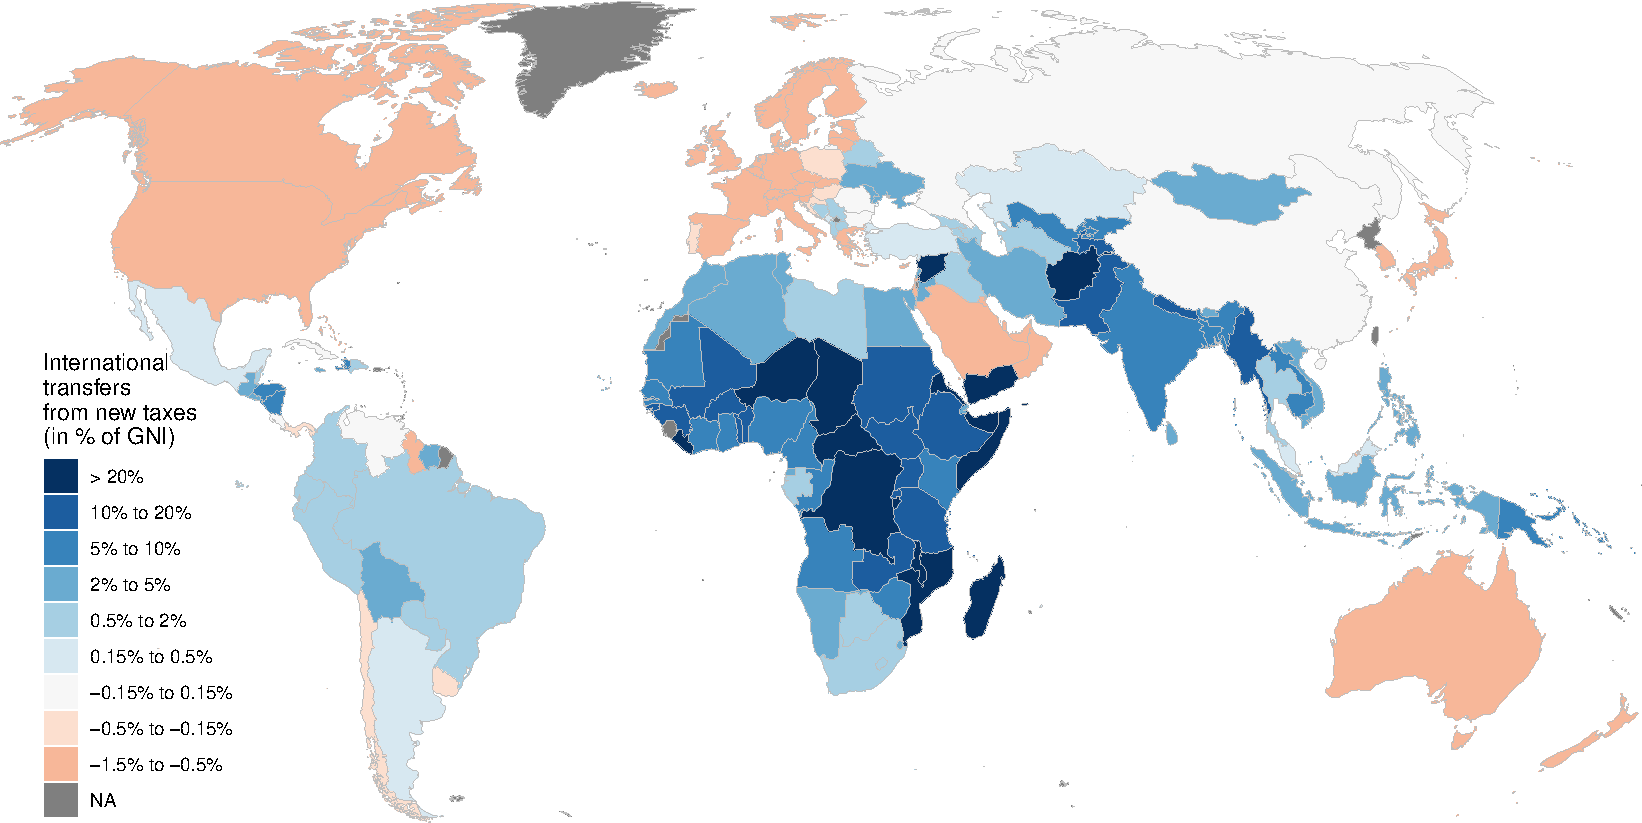
\includegraphics[width=1\textwidth]{../figures/maps/net_gain_over_gdp_both_taxes_pop.pdf}} 
\end{figure}

\clearpage
\begin{table}[!h]
  \caption{\label{tab:transfers_gain}Global taxes: international transfers, budget gain, revenues collected (\% of GNI). }
  \makebox[\textwidth][c]{
  
\begin{tabular}[t]{lccccccccc}
\toprule
  & \makecell{Int'l\\transfers} & \makecell{Budget\\gain} & \makecell{Wealth\\Tax (3\%\\$>$100M)} & \makecell{Wealth\\Tax (2\%\\$>$5M)} & \makecell{Fin.\\Trans.\\Tax} & \makecell{Carbon\\Tax\\(10\$/t)} & \makecell{Maritime\\fuel tax\\(100\$/t)} & \makecell{Aviation\\fuel tax\\(300\$/t)} & \makecell{Corporate\\inc. tax\\(min 21\%)}\\
\midrule
World & 0.0 & 3.2 & 0.72 & 1.28 & 0.32 & 0.33 & 0.10 & 0.22 & 0.3\\
Afghanistan & 47.6 & 50.3 & 0.29 & 0.49 & 0.58 & 0.88 & 0.01 & 0.42 & 0.0\\
DRC & 24.4 & 25.7 & 0.32 & 0.55 & 0.13 & 0.10 & 0.11 & 0.10 & 0.0\\
Sudan & 16.8 & 19.0 & 0.34 & 0.59 & 0.40 & 0.47 & 0.05 & 0.32 & 0.0\\
Uganda & 16.3 & 17.9 & 0.34 & 0.59 & 0.20 & 0.15 & 0.01 & 0.33 & 0.0\\
Myanmar & 15.8 & 18.0 & 0.36 & 0.61 & 0.51 & 0.35 & 0.04 & 0.25 & 0.0\\
Ethiopia & 14.7 & 16.4 & 0.35 & 0.60 & 0.14 & 0.12 & 0.00 & 0.45 & 0.0\\
Tanzania & 13.1 & 14.8 & 0.36 & 0.61 & 0.22 & 0.20 & 0.02 & 0.26 & 0.0\\
Pakistan & 11.3 & 12.4 & 0.02 & 0.05 & 0.35 & 0.49 & 0.04 & 0.18 & 0.0\\
Nigeria & 7.8 & 9.6 & 0.10 & 0.62 & 0.24 & 0.34 & 0.35 & 0.09 & 0.0\\
Kenya & 7.3 & 9.2 & 0.39 & 0.67 & 0.15 & 0.18 & 0.02 & 0.42 & 0.0\\
India & 6.3 & 10.2 & 1.26 & 1.51 & 0.26 & 0.61 & 0.05 & 0.17 & 0.0\\
Bangladesh & 5.9 & 6.4 & 0.03 & 0.06 & 0.13 & 0.17 & 0.02 & 0.08 & 0.0\\
Morocco & 4.1 & 6.6 & 0.44 & 0.74 & 0.23 & 0.49 & 0.18 & 0.46 & 0.0\\
Vietnam & 3.8 & 5.6 & 0.01 & 0.56 & 0.17 & 0.50 & 0.11 & 0.41 & 0.0\\
Egypt & 3.5 & 5.6 & 0.44 & 0.47 & 0.29 & 0.63 & 0.07 & 0.20 & 0.0\\
Philippines & 3.3 & 4.9 & 0.28 & 0.49 & 0.19 & 0.22 & 0.03 & 0.37 & 0.0\\
Iran & 3.0 & 6.9 & 0.45 & 0.77 & 0.37 & 1.63 & 0.39 & 0.22 & 0.0\\
Ukraine & 3.0 & 5.9 & 0.46 & 0.78 & 0.21 & 0.98 & 0.30 & 0.19 & 0.0\\
Indonesia & 2.9 & 4.8 & 0.25 & 0.41 & 0.23 & 0.45 & 0.23 & 0.32 & 0.0\\
Algeria & 2.5 & 5.1 & 0.46 & 0.78 & 0.26 & 0.72 & 0.18 & 0.14 & 0.0\\
Iraq & 1.8 & 5.9 & 0.47 & 0.80 & 0.33 & 1.00 & 1.34 & 0.09 & 0.0\\
Thailand & 1.6 & 4.8 & 0.49 & 0.83 & 0.25 & 0.61 & 0.20 & 0.79 & 0.0\\
Colombia & 1.6 & 4.0 & 0.49 & 0.83 & 0.20 & 0.24 & 0.36 & 0.30 & 0.0\\
South Africa & 1.6 & 5.6 & 0.33 & 0.64 & 0.19 & 1.12 & 0.53 & 0.38 & 0.8\\
Brazil & 0.8 & 3.7 & 0.60 & 0.78 & 0.17 & 0.29 & 0.57 & 0.23 & 0.2\\
Turkey & 0.5 & 2.0 & 0.13 & 0.23 & 0.24 & 0.45 & 0.10 & 0.37 & 0.0\\
Mexico & 0.2 & 2.2 & 0.59 & 0.73 & 0.17 & 0.30 & 0.05 & 0.22 & 0.0\\
Argentina & 0.2 & 2.5 & 0.54 & 0.92 & 0.15 & 0.35 & 0.18 & 0.23 & 0.0\\
China & -0.1 & 3.4 & 1.06 & 1.51 & 0.10 & 0.58 & 0.05 & 0.15 & 0.1\\
Russia & -0.1 & 3.1 & 0.87 & 1.06 & 0.18 & 0.79 & 0.16 & 0.24 & 0.0\\
Poland & -0.2 & 1.5 & 0.11 & 0.19 & 0.16 & 0.44 & 0.07 & 0.10 & 0.6\\
Saudi Arabia & -0.6 & 1.4 & 0.11 & 0.40 & 0.15 & 0.59 & 0.52 & 0.25 & 0.0\\
Spain & -0.6 & 1.1 & 0.24 & 0.40 & 0.22 & 0.14 & 0.06 & 0.37 & 0.3\\
Japan & -0.7 & 1.2 & 0.22 & 0.54 & 0.40 & 0.23 & 0.05 & 0.14 & 0.3\\
South Korea & -0.7 & 1.3 & 0.31 & 0.53 & 0.11 & 0.30 & 0.16 & 0.20 & 0.4\\
Italy & -0.8 & 0.8 & 0.35 & 0.50 & 0.17 & 0.13 & 0.04 & 0.15 & 0.2\\
United Kingdom & -0.8 & 3.2 & 0.25 & 0.43 & 2.36 & 0.12 & 0.04 & 0.28 & 0.6\\
Germany & -1.0 & 1.6 & 0.50 & 1.00 & 0.22 & 0.16 & 0.06 & 0.15 & 0.4\\
Canada & -1.0 & 2.4 & 0.59 & 1.25 & 0.09 & 0.27 & 0.08 & 0.26 & 0.9\\
France & -1.1 & 2.3 & 0.80 & 1.57 & 0.33 & 0.10 & 0.02 & 0.20 & 0.4\\
United States & -1.3 & 2.6 & 0.90 & 1.92 & 0.27 & 0.19 & 0.03 & 0.21 & 0.3\\
\bottomrule
\end{tabular} % add \midrule after World
} 
{\footnotesize \textit{Note:}  Budget gain denotes the sum of all other columns: international transfer and revenues collected. %revenue collected (last six columns) plus (net) international transfer (first column).
}
\end{table}
\clearpage

\begin{table}[!h]
  \vspace{-1cm}
  \caption{\label{tab:transfers_balance}Comparison of population vs. adult pop. entitlement; carbon balance (\% of GNI). }
  \makebox[\textwidth][c]{
  
\begin{tabular}[t]{lccccccc}
\toprule
  & \makecell{Int'l\\transfers\\(population)} & \makecell{Int'l\\transfers\\(adult)} & \makecell{Budget\\gain\\(population)} & \makecell{Budget\\gain\\(adult)} & \makecell{CO$_\text{2}$ balance\\\$185/tCO$_\text{2}$\\1990-2024} & \makecell{CO$_\text{2}$ balance\\discounted\\1990-2024} & \makecell{CO$_\text{2}$ balance\\discounted\\1850-2024}\\
\midrule
Afghanistan & 47.6 & 43.4 & 49.8 & 45.6 & 4748 & 3024 & 3361\\
DRC & 24.4 & 21.7 & 25.2 & 22.4 & 2721 & 1739 & 1907\\
Sudan & 16.8 & 15.6 & 18.4 & 17.2 & 1865 & 1156 & 1280\\
Uganda & 16.3 & 14.6 & 17.3 & 15.6 & 1755 & 1122 & 1226\\
Myanmar & 15.8 & 16.2 & 17.3 & 17.7 & 1996 & 1170 & 1389\\
Ethiopia & 14.7 & 13.7 & 15.8 & 14.8 & 1660 & 1047 & 1158\\
Tanzania & 13.1 & 11.9 & 14.2 & 12.9 & 1487 & 938 & 1033\\
Pakistan & 11.3 & 10.7 & 12.4 & 11.8 & 1122 & 699 & 784\\
Nigeria & 7.8 & 7.1 & 9.0 & 8.2 & 860 & 539 & 601\\
Kenya & 7.3 & 6.9 & 8.5 & 8.1 & 861 & 540 & 592\\
India & 6.3 & 6.4 & 8.7 & 8.8 & 650 & 383 & 456\\
Bangladesh & 5.9 & 6.0 & 6.4 & 6.4 & 749 & 448 & 517\\
Morocco & 4.1 & 4.1 & 5.9 & 5.9 & 435 & 254 & 308\\
Vietnam & 3.8 & 4.0 & 5.0 & 5.2 & 400 & 221 & 273\\
Egypt & 3.5 & 3.4 & 5.2 & 5.1 & 287 & 170 & 203\\
Philippines & 3.3 & 3.3 & 4.4 & 4.4 & 407 & 248 & 282\\
Iran & 3.0 & 3.1 & 6.1 & 6.2 & -276 & -190 & -180\\
Ukraine & 3.0 & 3.2 & 5.1 & 5.4 & -397 & -160 & -352\\
Indonesia & 2.9 & 2.9 & 4.4 & 4.5 & 282 & 165 & 203\\
Algeria & 2.5 & 2.5 & 4.3 & 4.3 & 111 & 66 & 83\\
Iraq & 1.8 & 1.7 & 5.1 & 4.9 & 4 & -10 & -3\\
Thailand & 1.6 & 1.8 & 4.0 & 4.1 & 54 & 20 & 52\\
Colombia & 1.6 & 1.7 & 3.2 & 3.3 & 221 & 133 & 154\\
South Africa & 1.6 & 1.6 & 5.0 & 5.0 & -295 & -168 & -199\\
Brazil & 0.8 & 0.9 & 2.9 & 3.0 & 135 & 77 & 95\\
Turkey & 0.5 & 0.5 & 1.8 & 1.8 & 7 & -2 & 9\\
Mexico & 0.2 & 0.2 & 1.5 & 1.5 & 15 & 12 & 14\\
Argentina & 0.2 & 0.2 & 1.6 & 1.6 & 8 & 3 & 8\\
China & -0.1 & -0.1 & 1.9 & 2.0 & -38 & -41 & -25\\
Russia & -0.1 & -0.1 & 2.1 & 2.1 & -329 & -179 & -247\\
Poland & -0.2 & -0.2 & 1.3 & 1.3 & -148 & -80 & -115\\
Saudi Arabia & -0.6 & -0.6 & 1.0 & 1.0 & -161 & -107 & -111\\
Spain & -0.6 & -0.6 & 0.7 & 0.7 & -35 & -16 & -16\\
Japan & -0.7 & -0.7 & 0.6 & 0.6 & -88 & -48 & -55\\
South Korea & -0.7 & -0.7 & 0.8 & 0.8 & -104 & -64 & -62\\
Italy & -0.8 & -0.8 & 0.3 & 0.3 & -43 & -19 & -23\\
United Kingdom & -0.8 & -0.8 & 2.8 & 2.8 & -45 & -21 & -38\\
Germany & -1.0 & -1.0 & 0.6 & 0.6 & -74 & -39 & -58\\
Canada & -1.0 & -1.0 & 1.2 & 1.2 & -122 & -69 & -83\\
France & -1.1 & -1.1 & 0.8 & 0.8 & -21 & -9 & -17\\
United States & -1.3 & -1.3 & 0.7 & 0.7 & -99 & -54 & -71\\
\bottomrule
\end{tabular} % add \midrule after World
} 
{\footnotesize \textit{Note:} Budget gain denotes the country net entitlements, i.e. the revenue it collects plus the net international transfer. International transfers denotes the country net entitlements minus taxes paid in the country. The carbon balance is separated from the tax proposals, it corresponds to the carbon credit or debt over 1850--2024 (or 1990--2024), priced at \$185/tCO$_\text{2}$ and annualized at 3.5\%. For example, a country with excess emissions compared to the world average accumulates a carbon debt. % Budget gain denotes the sum of all other columns: international transfer and revenues collected. %revenue collected (last six columns) plus (net) international transfer (first column).
}
\end{table}
\clearpage


\section{Wealth tax}\label{sec:wealth}

% Under its G20 presidency, Brazil commissionned a report on a global tax on ultra-high wealth. Indeed, the richest pay less taxes than average people in proportion to their contributive capacity, as most of their income is in the form of unrealized capital gains not subject to taxation. The report by \cite{zucman_blueprint_2024} proposes a top-up tax on the wealth of individual owning more than \$100 million, to collect the missing income tax revenue. With a 3\% top-up tax, a billionaire who already pays taxes amounting to 1\% of its wealth would be liable to an additional 2\% tax. Although a top-up tax may be 

We simulate two wealth taxes. First, a global tax on ultra-high wealth: a 3\% tax on all individual wealth in excess of \$100 million. Second, a national wealth tax: a 2\% tax on wealth in excess of \$5 million. These taxes add up,\footnote{For example, with a wealth of \$150 million, someone would pay each year a tax of 2.9\% on their wealth: 1\% from the tax on ultra-high wealth ($3\% \cdot \left(150-100\right)=1.5M$) and 1.9\% from the national wealth tax.% ($2\% \cdot \left(150-5\right)=2.9M$).
} so the highest marginal tax rate is 5\%.


The World Inequality Lab offers an \href{https://wid.world/world-wealth-tax-simulator/}{online simulator} to estimate the revenue collected by a custom wealth tax in each world region. Building on this work, we disaggregate the revenue estimates at the country level. Courtesy of Félix Bajard, we obtained the simulator's underlying data for 50 countries covering 95\% of global wealth tax revenue. To impute missing data, we predict the taxable base from a linear regression of the log of taxable base on the log of nominal GDP per capita, weighted by country population. 

Following \cite{zucman_blueprint_2024}, we assume 20\% of tax evasion. We also conservatively assume that asset prices would decline by 10\%. Half of the revenue from the global tax on ultra-high wealth would not be retained domestically but channeled into a fund to finance sustainable development. This fund would return revenues to countries with a per capita GNI below a threshold. We fix this eligibility threshold at twice the world average per capita GNI, or \$26,885 per year (in nominal terms). Finally, eligible countries receive a transfer per person %adult 
proportional to the difference between the threshold and their GNI per capita.


\section{Financial Transactions Tax}\label{sec:ftt}

\cite{pekanov_global_2019} estimate the revenues from a Financial Transactions Tax (FTT). Following the proposal by the European Commission (2011), they use a rate of 0.1\% of bonds and stocks and a rate of 0.01\% on derivatives. We use their baseline scenario, which assumes evasion rates of 15\% on bonds and stocks and 70\% on derivatives, together with an elasticity of trading volumes of $-$1.\footnote{The formula is: $\text{Revenue} = \text{tax rate} \cdot \text{volume} \cdot \text{evasion} \cdot \left(1 + \text{tax rate} / \text{transaction cost}\right)^\text{elasticity}$.} 

\cite{pekanov_global_2019} provide estimates at the global level and for 18 high-income countries. We allocate the global revenue that does not originate from these 18 countries to remaining countries, in proportion to their GDP. 22\% of world revenues would be collected in these remaining countries, with a revenue amounting to 0.1\% of their GDP (vs. 0.56\% of GDP for the 18 high-income countries).
% In these remaining countries, the FTT collects 22\% of the world total, and 0.1\% of these countries' GDP (vs. 0.56\% of GDP in the 18 high-income countries).


\section{Carbon price}\label{sec:carbon}

We model simulate the international transfers a \$100/tCO$_\text{2}$ carbon price applied to all non-LULUCF CO$_\text{2}$ emissions. At the global level, and neglecting behavioral responses, 0.33\% of the world nominal GDP would be collected. 
%Contrary to the other taxes studied here, the revenues of the carbon price are not entirely pooled at the global level. Instead, we assume that 0.2\% of each country's nominal GDP would be pooled and rebated to all countries in proportion to their adult population. With some exceptions (such as Ireland and Switzerland), the carbon price revenues would cover more than the transfer owed to the rest of the world, leaving revenues for domestic spending even in high-income countries.

\section{Maritime fuel levy}\label{sec:wealth}

We simulate the revenues of a \$100/tCO$_\text{2}$ levy on maritime fuel. The emissions from shipping by country are given by the simple average between the minimum and maximum estimates of \citet{dequiedt_navigating_2024}, who graciously provided the data. 

\section{Aviation fuel levy}\label{sec:wealth}

Using data from \cite{graver_co2_2018},\footnote{We use the data unadjusted for tourism.} we estimate the revenues from a tax on all flights (domestic and international). Due to complex climate effects such as contrails, aviation the global warming potential of aviation (GWP*$_\text{100}$) is 3 times the warming caused by its CO$_\text{2}$ emissions \citep{lee_contribution_2021}. To fully account for all effects on global warming, the carbon levy on aviation should be multiplied by that factor. Therefore, we simulate a \$300/tCO$_\text{2}$ tax on aviation fuel, comparable to the \$100/tCO$_\text{2}$ tax on maritime fuel. We use the 2018 data without adjusting for the expected increase in air traffic, and without adjusting for the decrease in traffic that would follow the tax.\footnote{More generally, we do not adjust for inflation or changes in volumes throughout this technical note. Figures are only provided to get ballpark estimates and cannot be very precise.}

\section{Higher minimum corporate income tax}

We estimate extra revenue by country if the internationally agreed minimum rate on corporate income tax was raised from 15\% to 21\%, with no carve-out. We use data from the \href{https://www.taxobservatory.eu/fr/base-de-donn%C3%A9es/the-tax-deficit-simulator/}{tax deficit simulator} from the EU Tax Observatory. These estimates are available for 45 countries (from OECD and the G20). We impute missing data only for three high-income countries (Iceland, Israel, New Zealand) and conservatively assume no extra revenue for other (developing) countries with missing data.

\section{Carbon balance}

On top of the proposed new taxes, we compute historical responsibilites for climate change. We define a carbon balance as the sum of a country's excess emissions compared to the world average, each year between 1850 and 2024, priced at $p=$ \$185/tCO$_\text{2}$ (which corresponds to the social cost of carbon according to \citealp{rennert_comprehensive_2022}). 
% We report the carbon balance over nominal GNI in 2025 country-by-country in Table \ref{tab:transfers_balance}.
In Table \ref{tab:transfers_balance}, we report the carbon balance annualized at a risk-adjusted discount rate of $r =$ 3.5\%. Denoting $e_t^c$ the emissions of country $c$ in year $t$, and $\pi_t^c$ its share of the world population at $t$, its annualized carbon balance over nominal GNI, $B_c$, is: $ B_c = r \cdot p \cdot \sum_{t=1850}^{2024} e_t^c - \pi_t^c \cdot \sum_c e_t^c / \text{GNI}_c^{2023}\text{.}$ Our computations are based on historical CO$_\text{2}$ emissions excluding LULUCF sector \citep{gutschow_country-resolved_2021}.

\clearpage

\textit{Our figures are fully reproducible from our data and code, openly availably on\\ \href{https://github.com/bixiou/global_tax_attitudes/code_global/new_taxes.R}{github.com/bixiou/global\_tax\_attitudes/code\_global/new\_taxes.R}. %We are here to feed the public debate on global redistribution. We welcome counter-proposals, criticisms and suggestions concerning (including pull requests).  
}


\begin{figure}[h!] 
    \caption{Net gain for state budgets from new taxes and international transfers (revenue plus net transfer).}\label{fig:budget_gain_both_taxes}
    \makebox[\textwidth][c]{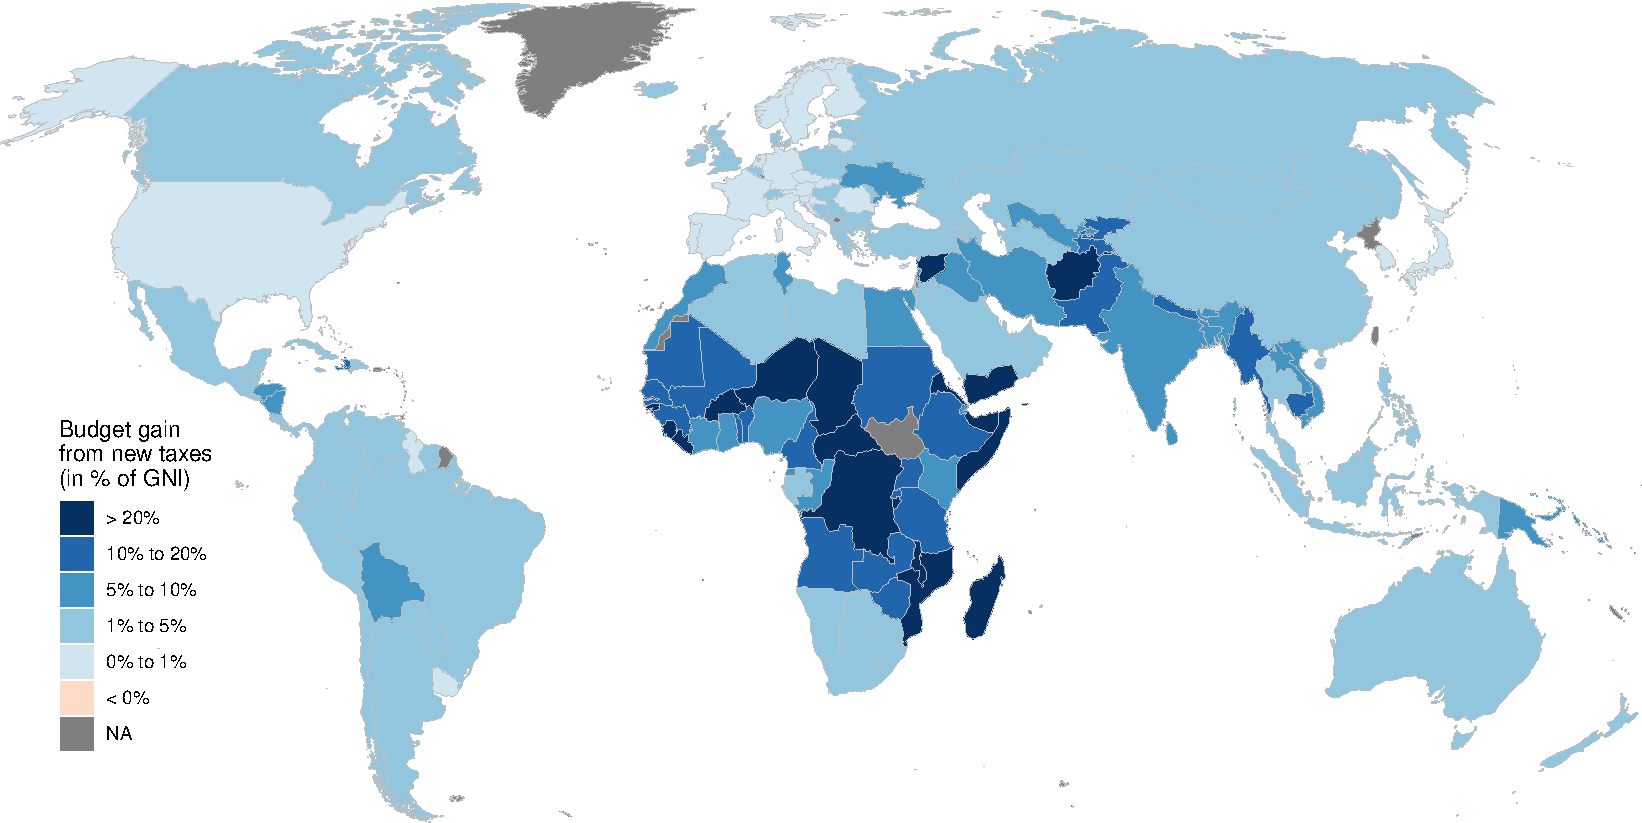
\includegraphics[width=.95\textwidth]{../figures/maps/budget_gain_over_gdp_both_taxes_pop.pdf}} 
\end{figure}
% {\footnotesize
% \begingroup
% \setstretch{.5}
% \titleformat*{\section}{\fontsize{11pt}{14pt}\bfseries\selectfont}
\renewcommand{\url}[1]{\href{#1}{Link}} % NCCcomment
\renewcommand\bibname{\small Bibliography}
\footnotesize
\bibliographystyle{plainnaturl_clean} % NCCcomment
\bibliography{global_tax_attitudes}
% \hphantom{\vphantom{
%     \begin{minipage}{\textwidth}
%         \bibliography{global_tax_attitudes}
%     \end{minipage}
% }}
% \endgroup }

\end{document}